% This is file JFM2esam.tex
%   (based on JFMsampl.tex v1.3 for LaTeX2.09)
% Copyright (C) 1996, 1997, 2014 Cambridge University Press
\documentclass{jfm}
\usepackage{graphicx}
\usepackage{braket}
\usepackage{tabularx}
\usepackage[dvipsnames]{xcolor}
\usepackage{url}
\usepackage{multirow}
\usepackage{hhline}
\usepackage{comment}
\usepackage{longtable}
\usepackage{booktabs}
\usepackage{subcaption}
\usepackage{float}
\usepackage[outdir=./]{epstopdf, epsfig}
\usepackage{wrapfig}
\usepackage[italian]{babel}

\setlength{\intextsep}{2pt}%
\setlength{\columnsep}{7pt}%

\title{Relazione di Laboratorio di Aerodinamica}
\shorttitle{Gruppo numero 08}
\shortauthor{Gruppo numero 08}

\author{
Anna Fontana\aff{1}, 
Giulio Gerardini\aff{2},\\
Aurora Orlandini\aff{3}, 
Alessandro Orseniga\aff{4}
}
\affiliation{
\aff{1} anna1.fontana@mail.polimi.it \& 280101 
\aff{2} giulio.gerardini@mail.polimi.it \& 280194 
\aff{3} aurora.orlandini@mail.polimi.it \& 271428
\aff{4} alessandro.orseniga@mail.polimi.it \& 270516
}
\date{22 Dicembre 2024}

\begin{document}

\maketitle

\section{Introduzione}
Lo scopo del progetto è studiare e confrontare le caratteristiche aerodinamiche dei profili NACA 0012, Althaus AH 79-100 C e quelle delle ali del Cessna 172 Skyhawk e del Lockheed U-2, le prime tramite l'utilizzo del metodo di Hess-Smith e di un apposito codice per il calcolo della linea media, le seconde tramite il metodo di Weissinger. La trattazione è basata sulle seguenti assunzioni: profili sottili, profili con bordo di uscita aperto, volto ad evitare oscillazioni del $C_p$, e ali piane ad alto allungamento. I risultati presentati sono stati ottenuti con MATLAB\textsuperscript{\textregistered} 2024b e XFOIL.

\section{Studio di profili alari}
\begin{wrapfigure}{r}{0.4\textwidth}
    \centering
    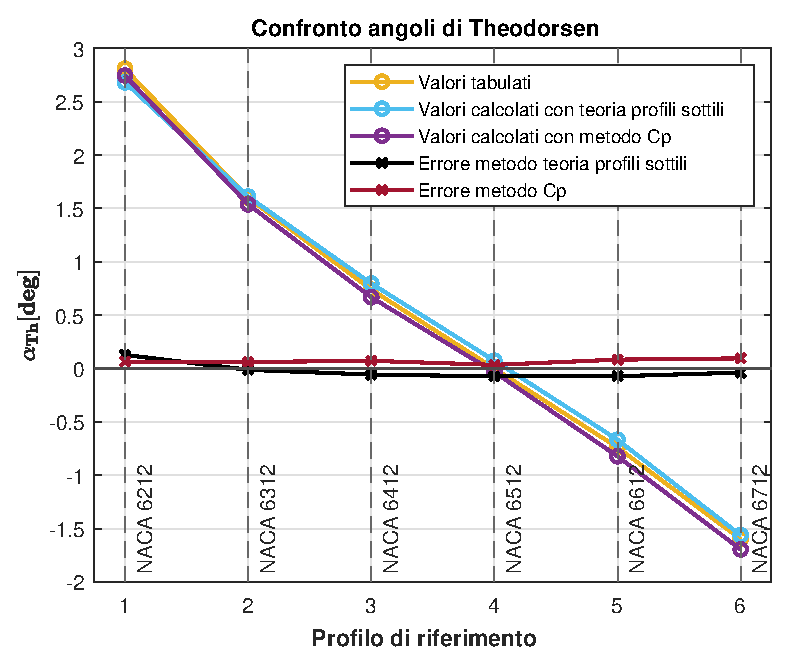
\includegraphics[width=\linewidth]{./figures/Theodorsen.eps}
    \caption{\textit{Errore massimo metodo geometrico: 0.1340$^{\circ}$. Errore massimo metodo $C_p$: 0.0950$^{\circ}$}}
    \label{fig:Theodorsen}
\end{wrapfigure}

Il codice di Hess-Smith è validato confrontando i valori ottenuti di $C_l$, $C_p$ e $C_m$ del NACA 0012, al variare del numero di pannelli da 100 a 364, con quelli restituiti da Xfoil, riscontrando una diminuzione progressiva degli errori. Il $C_p$ è ricavato utilizzando il teorema di Bernoulli con un errore massimo rispetto al risultato di XFOIL di $3.5\%$. Il $C_l$ è calcolato seguendo tre approcci diversi: tramite il teorema di Kutta-Joukowski, integrando il prodotto scalare della risultante delle forze di pressione agente su ciascun pannello e la normale alla velocità asintotica e seguendo l'approccio riportato in \cite{Foa}.
Il terzo metodo, con il quale la proiezione in direzione normale viene effettuata solo a seguito dell'integrazione, fornisce il risultato più simile a quello di XFOIL, effettuando meno operazioni nell'integrazione. Il $C_m$, risultante dall'integrazione del contributo di ciascun pannello, è ricavato al bordo d'attacco e trasportato poi ad $1/4$ della corda come in \cite{hs}. Si ottengono, per $\alpha$=2$^{\circ}$: $C_l=0.2416$, $C_m=-0.0028$ (errori del -0.04\% e 0.00\%).

L'angolo di progetto per i due profili è calcolato con due approcci. Tenendo presente la seguente definizione di linea media: \textit{il luogo dei punti situati a metà tra le  superfici di dorso e ventre lungo direzioni perpendicolari alla linea media stessa} \cite{Foa}, (tda), essa è calcolata con iterazioni di punto fisso usando un filtro di Savitzky–Golay per attenuare le oscillazioni numeriche. I parametri di tale metodo sono: il numero e la distribuzione di coordinate sul profilo, necessarie più fitte al bordo d'attacco, il polinomio interpolante, di tipo cubico Hermitiano, il numero di punti della linea media, pari a 1000, un quinto del quale pari all'ampiezza della finestra del filtro, la tolleranza sull'errore pari a $10^{-4}m$. Un approccio alternativo prevede lo studio dei picchi di $C_p$ sul bordo d'attacco al variare dell'angolo di incidenza: ridotto lo spessore del profilo al 10$\%$ di quello originario tramite XFOIL per rendere più evidente l'insorgere dei picchi, si sceglie l'angolo che induce quello di intensità minore. Per validare questi metodi i valori ottenuti sono confrontati con quelli riportati in \cite{TWS}.
Per il profilo Althaus si ottengono: 0.0370$^{\circ}$ (metodo $C_p$), -0.0191$^{\circ}$ (metodo geometrico), valori ritenuti plausibili e in accordo poichè prossimi allo stesso angolo ($0^{\circ}$). Per il profilo NACA 0012 si ottiene un angolo di $0.0000^{\circ}$.
\begin{figure}
\centering
    \begin{subfigure}{0.5\textwidth}
    \centering
        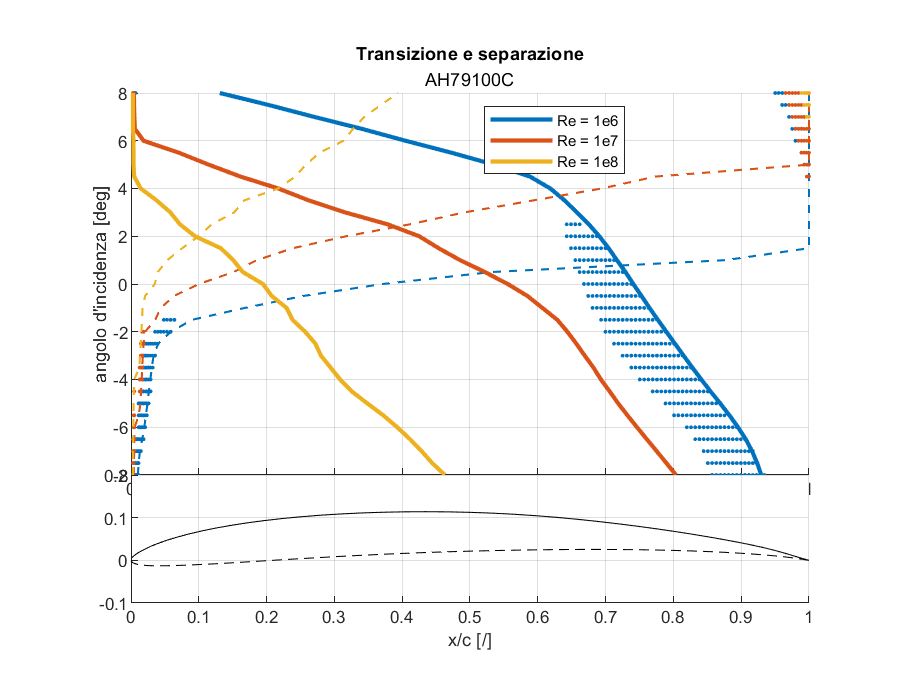
\includegraphics[width=\linewidth]{./figures/AH79100C.eps}
    \end{subfigure}%
    \begin{subfigure}{0.5\textwidth}
    \centering
        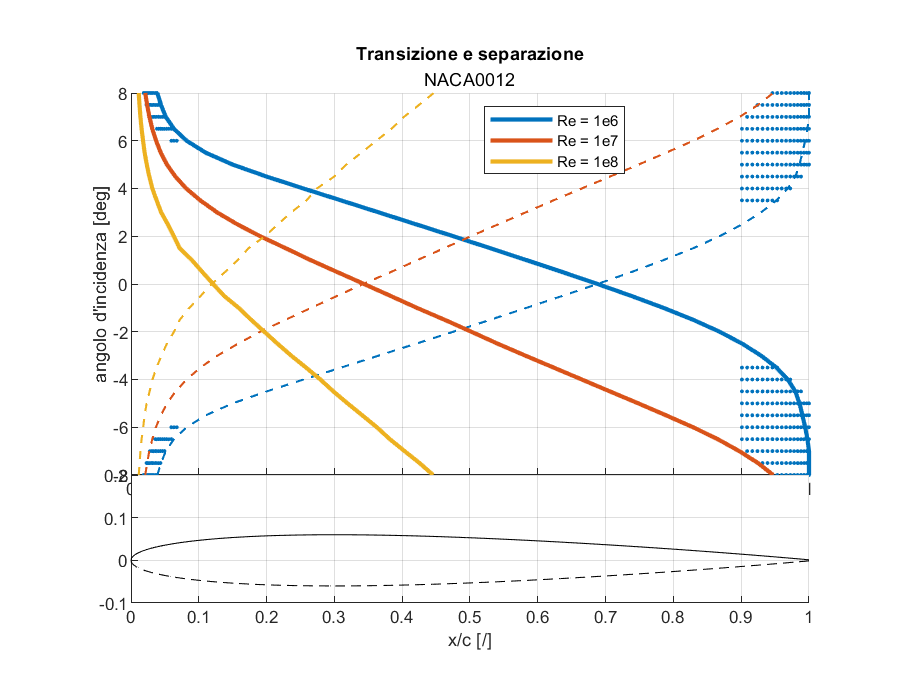
\includegraphics[width=\linewidth]{./figures/NACA0012.eps}
    \end{subfigure}
    \caption{\textit{Studio di transizione e separazione; la zona puntinata indica la separazione, le linee continue il punto di transizione sul dorso e quelle tratteggiate quello sul ventre.}}
    \label{fig:separazione}
\end{figure}
Transizione e separazione (studiata tramite il $C_f$) sono analizzate tramite XFOIL al variare di tre parametri: il numero di Reynolds tra $10^6$ e $10^8$, l'angolo di incidenza tra $-8^{\circ}$ e $8^{\circ}$ e il numero critico tra 8 e 10 (range scelti in base alle ipotesi del metodo e ai valori tipici delle applicazioni aeronautiche). Per entrambi i profili, a pari $Re$, all'aumentare di $N_{crit}$ la separazione si verifica ad angoli di attacco minori: lo strato limite ha minore quantità di moto ed è più incline alla separazione. Escludendo il bordo di uscita del NACA, essa avviene sempre in regime laminare e la corrente riattacca all'insorgere della transizione. A causa del camber del profilo Althaus, l'aumento di $\alpha$ comporta uno spostamento del punto di separazione verso il bordo d'attacco; comportamento quasi assente nel NACA. Per entrambi i profili, si riscontra separazione per $Re=10^6$, mentre per $Re$ superiori si verifica solo sul ventre dell'Althaus. Su di esso, a pari $\alpha$, questa avviene ad una percentuale di corda inferiore, per la presenza di un gradiente di pressione avverso anticipato da una più rapida riduzione della pendenza del dorso del profilo.
La transizione è anticipata, come previsto, al diminuire del numero critico. Confrontando i due profili a pari $\alpha$ (\figurename \ \ref{fig:separazione}), essa è anticipata nella prima porzione dell'Althaus e ritardata nella seconda. Rispetto al NACA, l'ascissa del punto di massimo camber del dorso è infatti più arretrata: la transizione risulta dunque mitigata dal gradiente di pressione favorevole agente nella prima porzione del profilo, ed è invece favorita nella zona di compressione (più marcata per via del camber).
\begin{comment}
Per il profilo NACA, essa si verifica solo per $Re=10^6$, mentre per l'Althaus avviene per $Re=10^6$ e solo sul ventre per $Re$ maggiori. . Mentre per il profilo NACA l'aumento dell'angolo di incidenza non influisce sul punto di separazione, per l'Althaus comporta un suo spostamento verso il bordo d'attacco, comportamento attribuibile all'elevato camber del profilo. Dato che la pendenza del dorso dell'Althaus decresce più rapidamente rispetto al NACA, la formazione del gradiente di pressione avverso è anticipata e per questo la separazione avviene a una percentuale di corda inferiore. Per entrambi i profili un aumento dell'angolo di incidenza comporta inoltre un avanzamento del punto di transizione verso il bordo di attacco. Dal confronto dei due grafici \figurename \ \ref{fig:separazione} si nota che a pari angolo di incidenza la transizione è ritardata dove la corrente è accelerante, nella zona del dorso ad inclinazione positiva, viceversa per la zona con un gradiente di pressione avverso. Per l'Althaus è quindi ritardata nella prima porzione di corda, ad inclinazione maggiore, e anticipata nella seconda rispetto al NACA.
\end{comment}

\section{Studio di piante alari di apertura finita}
Confrontando l'accuratezza delle implementazioni del metodo di Weissinger descritte in \cite{itca} e in \cite{ws} con la soluzione analitica di un'ala ellittica, si è deciso di adottare il primo metodo. 
\begin{comment}
\begin{wrapfigure}{l}{0.4\textwidth}
    \centering
    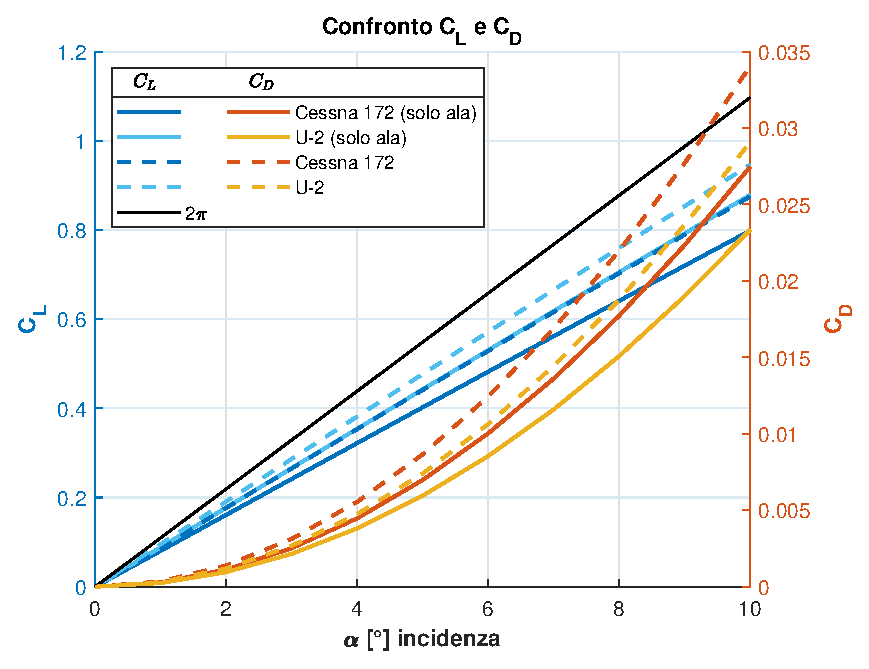
\includegraphics[width=\linewidth]{./figures/Ali_code_CL_CD.eps}
    \caption{}
    \label{fig:coefficienti}
\end{wrapfigure} 
\end{comment}
% \begin{comment}
\begin{figure}
\centering
    \begin{subfigure}{0.5\textwidth}
    \centering
        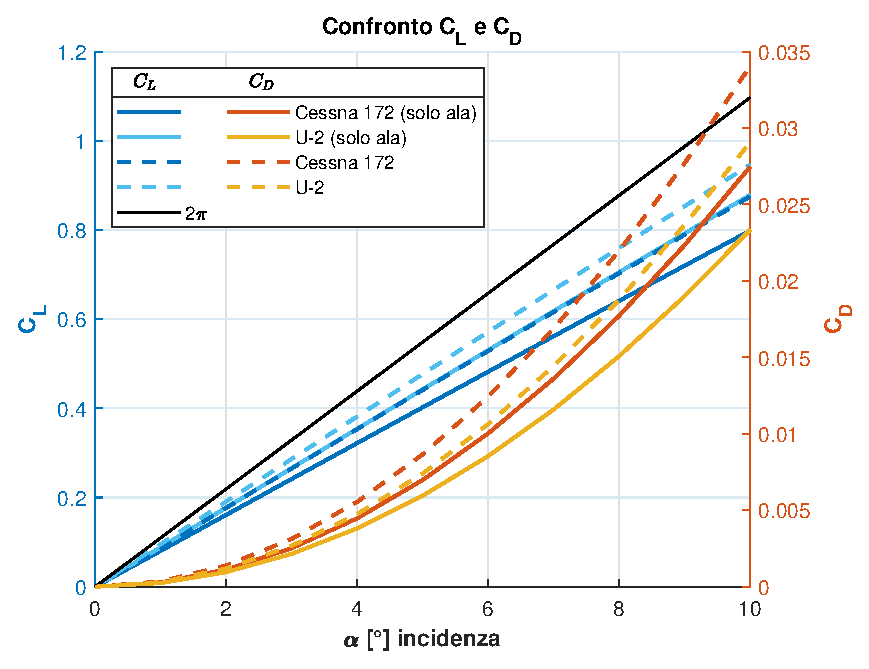
\includegraphics[width=\linewidth]{./figures/Ali_code_CL_CD.eps}
        
    \end{subfigure}%
    \begin{subfigure}{0.5\textwidth}
    \centering
        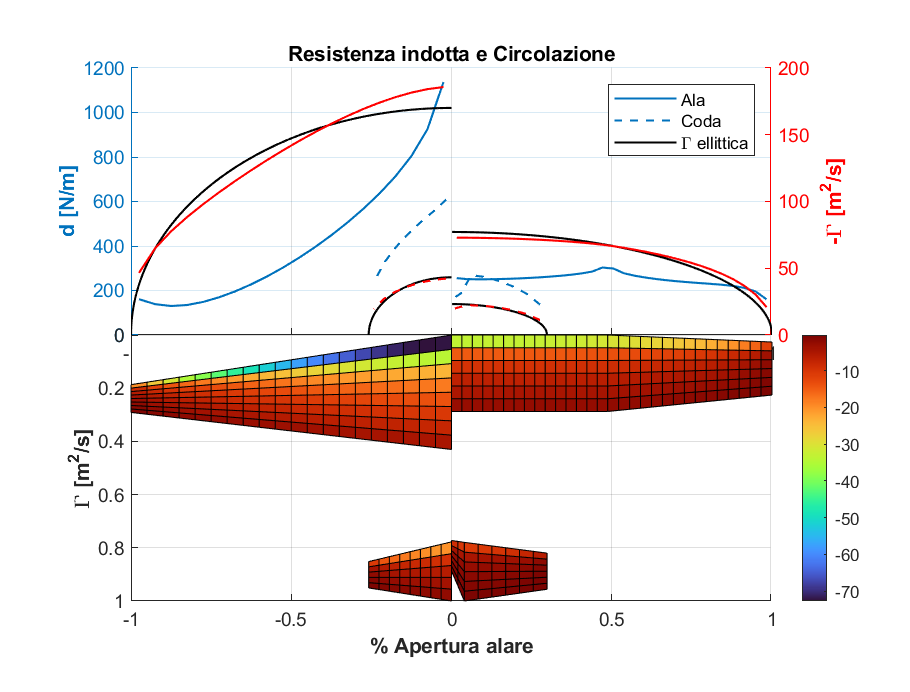
\includegraphics[width=\linewidth]{./figures/Distribuzioni_Ali_Code.eps}
    \end{subfigure}
    \caption{\textit{A sinistra confronto $C_L$ e $C_D$, a destra confronto resistenza indotta e circolazione}}
    
        \label{fig:coefficienti}
\end{figure}
% \end{comment}
L'aspect ratio del Lockheed U-2, pari a 10.52, è conforme alle ipotesi iniziali e superiore rispetto a quello del Cessna (7.32). Come si nota dalla \figurename \ \ref{fig:coefficienti}, a sinistra, questo influisce sulla pendenza della curva $C_{L/\alpha}$ (5.03 $rad^{-1}$ per l'U-2 e 4.57 $rad^{-1}$ per il Cessna) e sulla resistenza indotta, inferiore per il primo ma più regolare per il secondo, essendo la variazione di corda lungo l'apertura del Cessna costante lungo la prima metà e moderata successivamente. Tale distribuzione è influenzata anche dal taper ratio (0.24 per l'U-2 e 0.69 per il Cessna) e dall'angolo di freccia (7.56° e 3°): è quasi monotonicamente decrescente lungo l'apertura per il primo, mentre presenta un picco in corrispondenza della discontinuità geometrica per il secondo. 
Confrontando la circolazione generata dalle ali con una distribuzione ellittica che induca una pari portanza, si nota che quella del Cessna, per via della geometria non distante da quella ideale, è più prossima ad essa rispetto all'altro velivolo. Le polari riassumono quanto detto: tenendo conto del fatto che in questo modello la resistenza viscosa non è considerata, l'efficienza dell'U-2 è maggiore del $28.76\%$ rispetto a quella del Cessna considerando solo le ali e del $26.09\%$ considerando anche le code. L'U-2 presenta un $C_{L_{max}}$ maggiore (0.946 contro 0.875) e un $C_{D_{max}}$ minore (0.029 contro 0.034). L'aggiunta dei piani di coda causa, in entrambi i velivoli, un aumento del $C_L$ e del $C_D$ a parità di incidenza, effetti ragionevoli considerando l'aggiunta di una superficie portante.
\begin{comment}
\begin{wrapfigure}{r}{0.4\textwidth}
    \centering
    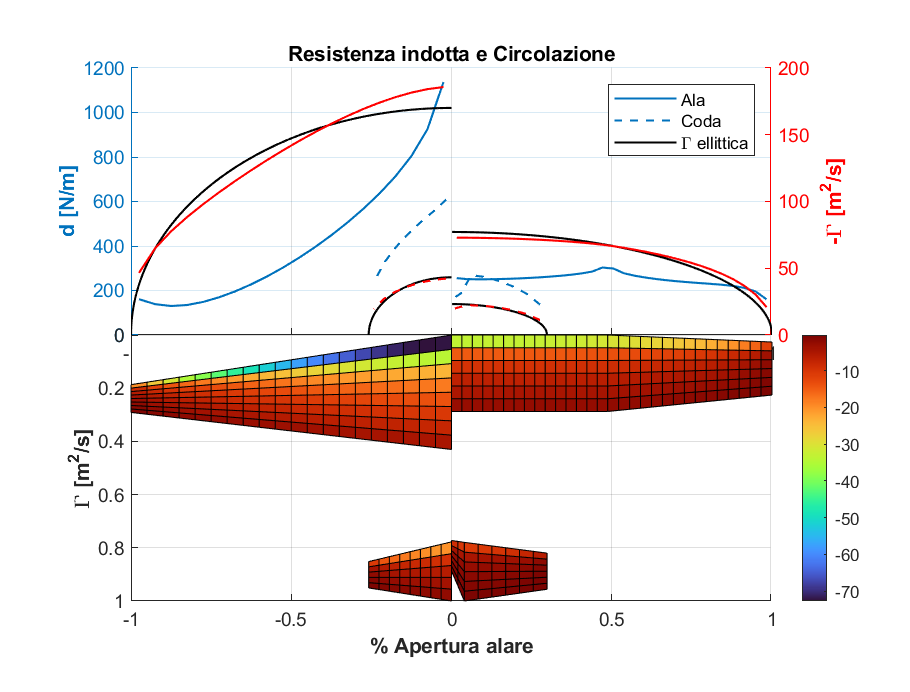
\includegraphics[width=\linewidth]{./figures/Distribuzioni_Ali_Code.eps}
    \caption{}
    \label{fig:Distribuzioni}
\end{wrapfigure} 
\end{comment}
Di conseguenza anche la pendenza della curva $C_{L_{\alpha}}$ aumenta (+9.61\% per il Cessna e +7.69\% per l'U-2), mentre l'efficienza massima diminuisce rispettivamente del $11.58\%$ e del $13.45\%$. Marginalmente (in media del $0.88\%$) aumenta anche la circolazione 2D sull'ala. \`E da considerare, tuttavia, che in questa trattazione è stata trascurata la necessità del centraggio del velivolo, ignorando quindi la possibilità di avere una coda deportante. I risultati ottenuti vanno interpretati alla luce di questo fatto e considerati non attendibili nel caso di coda deportante. 

\bibliographystyle{jfm}
\bibliography{ms}


  \ifnum\value{page}>3
    \section*{{\color{red} NUMERO DI PAGINE MAGGIORE DI 3! LAUREA REVOCATA!}}
  \fi  

\end{document}

